\documentclass[xcolor=table]{llncs}
\usepackage{booktabs}
\usepackage[table,xcdraw]{xcolor}
\usepackage[pdftex]{graphicx}  
\begin{document}
\title{Assigment 3 - Is it on cache?}
\author{Marco Espinoza \newline Jose Campos}
\institute{Instituto Tecnológico de Costa Rica}
\maketitle
\section{First reference misses}
The program main.c was executed 4 times using the program perf stat to track the number of cache references and cache misses during our main program execution. 
The results obtained are the following:
\begin{center}
\begin{table}[]
\centering
\caption{Perf stat results after 4 main program executions}
\label{table1}
\begin{tabular}{ccccccc}
\hline
\rowcolor[HTML]{000000} 
{\color[HTML]{FFFFFF} \textbf{\#}} & {\color[HTML]{FFFFFF} \textbf{\begin{tabular}[c]{@{}c@{}}Time elapsed \\ (ms)\end{tabular}}} & {\color[HTML]{FFFFFF} \textbf{\begin{tabular}[c]{@{}c@{}}Task-clock \\ (msec)\end{tabular}}} & {\color[HTML]{FFFFFF} \textbf{cycles}} & {\color[HTML]{FFFFFF} \textbf{instructions}} & {\color[HTML]{FFFFFF} \textbf{cache-references}} & {\color[HTML]{FFFFFF} \textbf{cache-misses}} \\ \hline
1 & 10,909 & 0,267 & 630722 & 423164 & 22265 & 10477 \\
2 & 0,446 & 0,202 & 595425 & 420416 & 22047 & 5813 \\
3 & 0,389 & 0,192 & 529091 & 426025 & 23513 & 2800 \\
4 & 0,487 & 0,223 & 517475 & 425037 & 21689 & 1907 \\ \hline
\end{tabular}
\end{table}
\end{center}
%
\subsection{Questions}
%
a. Why did the first run of your application report a high cache miss rate?\newline
Reason of this is because during the first execution the program is stored in the hard drive, and it is not loaded in the main memory or in the L2 cache.
It produces the core must to move the data from the drive to the cache, and it produces misses during the program execution.\newline\newline
b. Why did any subsequent execution report a decremental cache miss rate?\newline
Because after the first execution, part of the program is stored in the L2 cache, and it produces hits during the second or the next program executions, and as the program is being executed multiple times, due to the locality of reference, the number of misses is reduced.\newline
Those locality of reference consists on temporal and spacial locality, where the temporal locality refers to the reuse of specific data, and/or resources, within a relatively small time duration. Spatial locality refers to the use of data elements within relatively close storage locations memory.\newline
For those reasons the number of cache miss rate is reduced after the subsequent program execution.
\newline
%
\section{Optimizing memory accesses on loops}
%
On this section, the main application located into the part\_2 directory of the project files was used to be compiled through 2 kind of memory ordering, row and columns. 
The program was executed using both methods 5 times using perf stat to compare both results in terms of cache memory access. The results will be exposed in the following sections.\newline
\subsection{Row results}
The results obtained for the row results are presented in the next table.
\begin{table}[]
\centering
\caption{Perf stat results using row ordering during 5 times}
\label{table2}
\begin{tabular}{ccccccc}
\hline
\rowcolor[HTML]{000000} 
{\color[HTML]{FFFFFF} \textbf{\#}} & {\color[HTML]{FFFFFF} \textbf{\begin{tabular}[c]{@{}c@{}}Time elapsed \\ (ms)\end{tabular}}} & {\color[HTML]{FFFFFF} \textbf{\begin{tabular}[c]{@{}c@{}}Task-clock \\ (msec)\end{tabular}}} & {\color[HTML]{FFFFFF} \textbf{cycles}} & {\color[HTML]{FFFFFF} \textbf{instructions}} & {\color[HTML]{FFFFFF} \textbf{cache-references}} & {\color[HTML]{FFFFFF} \textbf{cache-misses}} \\ \hline
1                                  & 134.57                                                                                       & 4.583                                                                                        & 11628737                               & 24742637                                     & 202382                                           & 121747                                       \\
2                                  & 4.174                                                                                        & 3.894                                                                                        & 10964320                               & 24591759                                     & 150668                                           & 59725                                        \\
3                                  & 7.578                                                                                        & 7.061                                                                                        & 11608162                               & 24534858                                     & 153962                                           & 86481                                        \\
4                                  & 27.237                                                                                       & 4.173                                                                                        & 11261520                               & 24515829                                     & 148946                                           & 77911                                        \\
5                                  & 15.436                                                                                       & 3.953                                                                                        & 11056268                               & 24542301                                     & 155608                                           & 76989                                        \\ \hline
\end{tabular}
\end{table}\newline\newline
\subsection{Column results}
The results obtained for the column results are presented in the table 3.
\begin{table}[]
\centering
\caption{Perf stat results using row ordering during 5 times}
\label{table3}
\begin{tabular}{ccccccc}
\hline
\rowcolor[HTML]{000000} 
{\color[HTML]{FFFFFF} \textbf{\#}} & {\color[HTML]{FFFFFF} \textbf{\begin{tabular}[c]{@{}c@{}}Time elapsed \\ (ms)\end{tabular}}} & {\color[HTML]{FFFFFF} \textbf{\begin{tabular}[c]{@{}c@{}}Task-clock \\ (msec)\end{tabular}}} & {\color[HTML]{FFFFFF} \textbf{cycles}} & {\color[HTML]{FFFFFF} \textbf{instructions}} & {\color[HTML]{FFFFFF} \textbf{cache-references}} & {\color[HTML]{FFFFFF} \textbf{cache-misses}} \\ \hline
1                                  & 57.02                                                                                        & 5.117                                                                                        & 13173982                               & 24687156                                     & 258039                                           & 122711                                       \\
2                                  & 4.549                                                                                        & 4.25                                                                                         & 12371551                               & 24591174                                     & 206147                                           & 59734                                        \\
3                                  & 35.83                                                                                        & 4.42                                                                                         & 12422663                               & 24580902                                     & 212715                                           & 79864                                        \\
4                                  & 17.95                                                                                        & 4.803                                                                                        & 13089132                               & 24571754                                     & 237982                                           & 85326                                        \\
\multicolumn{1}{l}{5}              & 21.60                                                                                        & 4.45                                                                                         & 12696407                               & 24502248                                     & 232095                                           & 78962                                        \\ \hline
\end{tabular}
\end{table}
\subsection{Questions}
\paragraph{}
a. What kind of optimization is performed on the program?\newline
The kind of optimization performed on the program is called permutation. Loop permutation takes advantage of the memory ordering used by an specific programming language for data allocation improving data locality. The followed image present both examples used on this section, row and column ordering.\newline
\begin{figure}
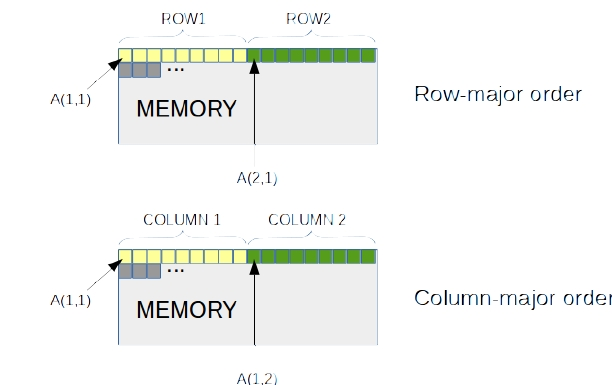
\includegraphics[scale=0.4]{row_column.jpg}
\centering
\caption{Figure1}
\label{fig: Row and Column ordering implemented in the section 2}
\end{figure}\newline
\paragraph{}
b. Why does the cache miss rate is higher for the row results? Is this expected according to the loop optimizations implemented? Provide detail on your thoughts.\newline
\paragraph{}
Because with the row implementation, during each iteration, the program is accessing the next cache line, increasing the probability to have misses, because when the next cache line is accessed, it is possible the old cache line could be replaced for a new data because the program will continue moving trough the cache lines. As result, when a data which is stored in the old cache lines is required, it could be possible the data is not in the L2, and the core will require to wait until the data is again in the L2, producing a higher miss rate compared with the column ordering\newline
The next table presents the miss-rate for both orderings.
\begin{table}[htbp]
\centering
\caption{Row miss rate vs Column miss rate}
\label{table4}
\begin{tabular}{ccccccc}
\hline
\rowcolor[HTML]{000000} 
{\color[HTML]{FFFFFF} \textbf{\#}} & {\color[HTML]{FFFFFF} \textbf{\begin{tabular}[c]{@{}c@{}}Time elapsed \\ (ms)\end{tabular}}} & {\color[HTML]{FFFFFF} \textbf{\begin{tabular}[c]{@{}c@{}}Task-clock \\ (msec)\end{tabular}}} & {\color[HTML]{FFFFFF} \textbf{cycles}} & {\color[HTML]{FFFFFF} \textbf{instructions}} & {\color[HTML]{FFFFFF} \textbf{cache-references}} & {\color[HTML]{FFFFFF} \textbf{cache-misses}} \\ \hline
1 & 10,909 & 0,267 & 630722 & 423164 & 22265 & 10477 \\
2 & 0,446 & 0,202 & 595425 & 420416 & 22047 & 5813 \\
3 & 0,389 & 0,192 & 529091 & 426025 & 23513 & 2800 \\
4 & 0,487 & 0,223 & 517475 & 425037 & 21689 & 1907 \\ \hline
\end{tabular}
\end{table} 
\newline
\newline
\newline
\paragraph{}
c. Why do the cache references are higher for the column results? Provide detail on your thoughts.\newline
The cache references is higher for the column results due to during each iteration, the same cache line is accessed, and it helps to increase the number of hits due to the special locality. Because the program is accessing addresses belonging to the same cache line, and it increments the probability to continue accessing addresses close to the current address. 
The following table shows the results for the cache references obtained in both methods. 
\begin{table}[]
\centering
\caption{Column cache references between Row cache references}
\label{table4}
\begin{tabular}{ccc}
\hline
\rowcolor[HTML]{000000} 
{\color[HTML]{FFFFFF} \textbf{\#}} & {\color[HTML]{FFFFFF} \textbf{Column Cache-References}} & {\color[HTML]{FFFFFF} \textbf{Row Cache References}} \\ \hline
1 & 258039 & 202382 \\
2 & 206147 & 150668 \\
3 & 212715 & 153962 \\
4 & 237982 & 148946 \\
5 & 232095 & 155608 \\ \hline
\end{tabular}
\end{table}
\newline
\paragraph{}
d. Why do the cache misses are similar between both tests? Is this expected according to the loop optimization method implemented? Provide detail on
your thoughts.\newline
e. How is the loop optimization related to the instructions per cycle reported for each test case ( insns per cycle) ?\newline
%
\end{document}
